% *********************************************************************
% © 2016–2026 Jeremy Sylvestre
%
% Permission is granted to copy, distribute and/or modify this document
% under the terms of the GNU Free Documentation License, Version 1.3 or
% any later version published by the Free Software Foundation; with no
% Invariant Sections, no Front-Cover Texts, and no Back-Cover Texts. A
% copy of the license is included in the appendix entitled “GNU Free
% Documentation License” that appears in the output document of this
% PreTeXt source code. All trademarks™ are the registered® marks of
% their respective owners.
%
% *********************************************************************
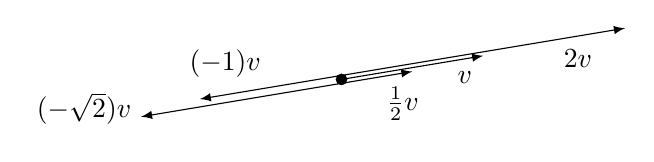
\begin{tikzpicture}[
	point/.style={circle,draw,very thin,fill,inner sep=0pt,minimum size=4pt},
	vector/.style={-latex},
]
	\node[point] at (0,0) {};
	\draw[vector] (0,0) to node[below right,near end] {$\uvec{v}$} (1.8,0.3);
	\draw[vector] (0,0.05) to node[below right,near end] {$2 \uvec{v}$} (3.6,0.65);
	\draw[vector] (0,-0.05) to node[below right] {$\frac{1}{2} \uvec{v}$} (0.9,0.1);
	\draw[vector] (0,0.05) to node[above left] {$(-1) \uvec{v}$} (-1.8,-0.25);
	\draw[vector] (0,-0.05) to node[left,at end,yshift=0.1cm] {$(-\sqrt{2}) \uvec{v}$} (-2.546,-0.474);
\end{tikzpicture}
